\section{Proposed Federated DDQN Offloading Framework}
\label{sec:fed_ddqn}

\subsection{MDP Definition}

The Stage-1 scheduler is formulated as an offline replay MDP over the fixed \dataset{} sequence. At each decision step, the agent observes a feature vector $x_i\in\mathbb{R}^{30}$ derived from task, edge, network, and cloud state. It selects action $a_i\in\{0,1\}$, receives reward $r_i$, and then advances to the next sampled task state. The next state is exogenous in the benchmark: selecting edge or cloud changes the reward assigned to the current task, but it does not mutate the CSV queue state for the following timestep during training. The state includes task demand and urgency, local edge availability, queue pressure, channel indicators, and cloud load indicators. It does not include artificial sentinel values for rejected tasks.

The action space is intentionally binary. Edge execution is selected by $a_i=0$ and cloud execution by $a_i=1$. A rejected task is a failure outcome after feasibility checks, not a choice the policy can make. This makes the comparison stricter. The policy must decide where to execute the task, and it is penalized if that destination leads to infeasibility or SLA failure.

\subsection{DDQN and Dueling Q-Network}

The proposed policy uses a Double DQN target:
\begin{equation}
y_i=r_i+\gamma\left(1-\zeta_i^{\mathrm{term}}\right)
Q_{\theta^-}\left(x_{i+1},\arg\max_{a'}Q_{\theta}(x_{i+1},a')\right),
\label{eq:ddqn_target_main}
\end{equation}
where $\theta$ are the online network parameters, $\theta^-$ are the target network parameters, and $\zeta_i^{\mathrm{term}}$ is a binary terminal-mask indicator. The mask is one at sequence ends, purged split or gap boundaries, and final-sample boundaries where bootstrapping should not cross into another evaluation interval. The loss is the Huber temporal-difference loss between $Q_\theta(x_i,a_i)$ and $y_i$. In the present offline benchmark, the next state remains exogenous and precomputed; the terminal mask defines where value bootstrapping is conceptually suppressed, not where an online simulator resets because of the selected action.

The Q-network uses a dueling architecture:
\begin{equation}
Q(x,a)=V(x)+A(x,a)-\frac{1}{|\mathcal{A}|}\sum_{a'\in\mathcal{A}}A(x,a').
\label{eq:dueling_main}
\end{equation}
The value stream estimates the quality of the state, while the advantage stream estimates the relative value of edge versus cloud. This separation helps when task urgency or network degradation dominates the decision regardless of the final action.

\subsection{Reward Design}

The reward follows the final evaluation metrics. A simplified form is
\begin{equation}
r_i = -\alpha_L \tilde{L}_i - \alpha_S M_i - \alpha_R R_i
      - \alpha_E P^e_i - \alpha_H H_i,
\label{eq:reward}
\end{equation}
where $\tilde{L}_i$ is normalized selected latency, $M_i$ indicates SLA miss, $R_i=F_i$ indicates selected-path rejection or admission failure, $P_i^e$ is edge pressure or edge-overuse cost, and $H_i$ penalizes routing heavy AI, video, image, or firmware-like tasks to edge when cloud is clearly better. The reward does not force a permanent preference for edge or cloud. It makes a poor destination costly for the reason it is poor: latency, SLA miss, rejection, overload, or heavy-task mismatch.

Because $R_i$ is defined as feasibility/admission failure rather than $M_i\lor F_i$, an SLA miss and a rejection are not automatically double-counted. A task receives both penalties only when the selected path both misses its deadline and fails the feasibility/admission predicate.

For reward shaping, $L_i^{\mathrm{best}}$ and $L_i^{\mathrm{worst}}$ denote the minimum and maximum finite generated latency over the edge and cloud alternatives after infeasible sentinel values are excluded. The regret term uses the same normalized selected-latency scale as $\tilde{L}_i$.

\begin{table*}[!t]
\centering
\caption{Reward components used to align Fed-DDQN training with final QoS evaluation.}
\label{tab:reward_terms}
\scriptsize
\begin{tabularx}{\textwidth}{@{}lXX@{}}
\toprule
Term & Meaning & Intended behavior \\
\midrule
$-\alpha_L \tilde{L}_i$ & Normalized selected latency penalty. & Prefer lower-latency edge or cloud decisions. \\
$-\alpha_S M_i$ & SLA miss penalty. & Discourage choices that violate task-specific deadlines. \\
$-\alpha_R R_i$ & Rejection/admission penalty. & Penalize selected-path resource, security, battery, corruption, or destination-state infeasibility. \\
$-\alpha_E P_i^e$ & Edge pressure or edge-overuse penalty. & Prevent the policy from routing too much work to constrained edge nodes. \\
$-\alpha_H H_i$ & Heavy-task misrouting penalty for AI, video, image, and firmware-like tasks. & Shift large or cloud-favorable workloads away from edge when local execution is not actually better. \\
\bottomrule
\end{tabularx}
\end{table*}

\begin{table*}[!t]
\centering
\caption{Reward and model-selection details used for reproducibility.}
\label{tab:reward_reproducibility}
\scriptsize
\begin{tabularx}{\textwidth}{@{}lXXc@{}}
\toprule
Component & Implemented form & Purpose & Status \\
\midrule
Latency shaping & $1.25\{1-2(L_i-L_i^{\mathrm{best}})/(L_i^{\mathrm{worst}}-L_i^{\mathrm{best}}+\epsilon)\}$ & Rewards lower selected latency relative to the edge/cloud alternatives. & Fixed \\
Regret penalty & $-0.75\,\mathrm{clip}(L_i-L_i^{\mathrm{best}},0,2)$ after normalization & Penalizes choosing a destination far from the better generated alternative. & Fixed \\
SLA margin & Positive margin weight $1.05$; negative margin weight $2.10$ & Makes deadline misses more costly than equal-sized positive slack is beneficial. & Fixed \\
Rejection/admission & $-2.25$ when selected path is infeasible or a deadline-admission flag applies & Aligns training with selected-path rejection reporting. & Fixed \\
Heavy-task edge misuse & Penalty for heavy AI, video, image, and firmware-like tasks routed to edge when cloud is not worse & Reduces edge bias for cloud-favorable heavy workloads. & Fixed \\
Energy and battery shaping & Small energy requirement penalty and low-battery non-urgent penalty & Discourages avoidable edge use under device pressure. & Fixed \\
Reward clipping & Final reward clipped to $[-5,5]$ & Prevents rare generated extremes from dominating replay updates. & Fixed \\
Validation score & $\bar{L}+5.0M_{\mathrm{SLA}}+2.5R+0.8[U^e-78]_+ +1.2H$ & Selects the checkpoint by latency, SLA, rejection, edge balance, and heavy-task behavior. & Validation-selected \\
\bottomrule
\end{tabularx}
\end{table*}


The reward design controls the edge bias that can appear when a learner overvalues local execution for tight-deadline tasks. Prioritized replay \cite{ref37} and stronger action-aware pressure are diagnostic variants, but the proposed configuration uses standard replay, light FedProx regularization, an explicit validation penalty for excessive edge usage, and a heavy-task penalty. These choices keep the model within the Fed-DDQN family while discouraging the policy from routing large cloud-favorable tasks to constrained edge nodes.

\subsection{Channel-Aware Decision Margin}

The binary action is simple, but the decision boundary is not. The learned Q-values can be read through a decision margin
\begin{equation}
\Delta Q_i = Q_{\theta}(x_i,\mathrm{edge}) - Q_{\theta}(x_i,\mathrm{cloud}).
\label{eq:q_margin}
\end{equation}
The policy selects edge when $\Delta Q_i>0$ and cloud otherwise. The margin connects the neural decision to the physical factors in the state vector. A compact hand-written proxy for the same intuition separates edge-side and cloud-side penalties on a normalized score scale:
\begin{align}
\widehat{S}_i^e &=
\tilde{L}_i^e+\beta_q\tilde{q}^e_{j_i,t_i}+\beta_h h_i, \\
\widehat{S}_i^c &=
\tilde{L}_i^c+\beta_\ell \ell_{t_i}+\beta_o o_{t_i}+\beta_\xi \xi_{t_i}, \\
\Delta S_i &= \widehat{S}_i^c-\widehat{S}_i^e.
\label{eq:latency_margin}
\end{align}
Here $\tilde{L}_i^e$ and $\tilde{L}_i^c$ are normalized generated latency terms, $\tilde{q}^e_{j_i,t_i}$ is normalized local queue pressure, and the $\beta$ coefficients are dimensionless interpretive weights. The terms $h_i$, $\ell_{t_i}$, $o_{t_i}$, and $\xi_{t_i}$ represent heavy-task mismatch, packet loss, outage, and jitter/congestion stress. This proxy is illustrative only; reported decisions are produced by the learned Q-network, not by this hand-written score. It describes the kind of nonlinear boundary the network must learn: edge is attractive when the adjusted cloud path is more expensive, but that advantage should shrink when local queue pressure or heavy-task mismatch raises the edge-side cost. For this reason, the state contains both task descriptors and channel/resource indicators, and the final evaluation reports action distribution and scenario behavior instead of relying only on average latency.

\subsection{Zone-Based Federated Training}

The dataset is partitioned into edge zones. Each zone trains a local DDQN model on its own non-identical distribution. After local updates, the server aggregates zone models using weighted FedAvg:
\begin{equation}
\theta^{(r+1)}=\sum_{z=1}^{Z}\frac{n_z}{\sum_{k=1}^{Z}n_k}\theta_z^{(r+1)},
\label{eq:fedavg_main}
\end{equation}
where $n_z$ is the number of samples used by zone $z$. This weighting prevents small zones from dominating the global update while still allowing their local behavior to influence the shared model.

FedProx regularization is used to reduce excessive local drift:
\begin{equation}
\mathcal{L}_z=\mathcal{L}_{\mathrm{TD},z}+\frac{\mu}{2}\lVert\theta_z-\theta_g\rVert_2^2.
\label{eq:fedprox_main}
\end{equation}
The final implementation uses $\mu=0.003$ with a drift clamp to avoid numerically unstable local-drift values. The proximal term is light enough to allow local adaptation but strong enough to discourage zone models from moving too far away from the current global policy.

\begin{figure*}[!t]
\centering
\fbox{\begin{minipage}{0.95\textwidth}
\textbf{Algorithm 1: Zone-Aware Federated DDQN Training}\\[0.35em]
\textbf{Input:} train split, zone partitions, global network $Q_{\theta}$, target network $Q_{\theta^-}$, replay buffers, maximum rounds.\\
\textbf{Output:} validation-selected global policy.\\[0.35em]
1) Initialize the global dueling DDQN and broadcast its weights to all active edge-zone clients.\\
2) For each federated round, sample local training transitions within each zone and update the local online network with the terminal-masked DDQN target in \eqref{eq:ddqn_target_main}.\\
3) Add the FedProx drift penalty in \eqref{eq:fedprox_main} using the current global model as the anchor.\\
4) Clip or sanitize unstable drift values before the optimizer step, matching the final numerically stable training path.\\
5) Return local model weights and sample counts from each zone.\\
6) Aggregate local models by weighted FedAvg as in \eqref{eq:fedavg_main}.\\
7) Evaluate the global model on the validation interval. Save the best checkpoint by the validation score in \eqref{eq:validation_score_main}.\\
8) Stop when patience is reached or the maximum number of rounds is exhausted. Restore the best global checkpoint before test evaluation.
\end{minipage}}
\caption{Training procedure for the proposed \fedddqn{} policy. The test split is not used inside the training loop.}
\label{alg:fed_ddqn_training}
\end{figure*}


\subsection{Validation Checkpointing}

Model selection uses the validation interval, not the test interval. The validation score is
\begin{equation}
\begin{aligned}
S_{\mathrm{val}}={}&
\bar{L}_{\mathrm{val}}
 + 5.0 M_{\mathrm{SLA,val}}
 + 2.5 R_{\mathrm{val}} \\
&+ 0.8 \left[U^e_{\mathrm{val}}-78\right]_+
 + 1.2 H_{\mathrm{val}} .
\end{aligned}
\label{eq:validation_score_main}
\end{equation}
where $\bar{L}_{\mathrm{val}}$ is average validation latency in milliseconds, $M_{\mathrm{SLA,val}}$ is SLA miss percentage, $R_{\mathrm{val}}$ is rejection percentage, $U^e_{\mathrm{val}}$ is validation edge usage percentage, and $H_{\mathrm{val}}$ is the percentage of heavy cloud-favorable tasks routed to edge. The operator $[x]_+=\max(x,0)$ applies the edge-overuse penalty only above the 78\% soft cap. Percentages are expressed as percentage points in $[0,100]$, so the coefficients have units of milliseconds per percentage point. The best global model is restored before final test evaluation. The final training run selected validation round \FedBestValRound{} with score \FedBestValScore{}, and training ran for \FedRoundsRan{} rounds before stopping.

\begin{figure*}[!t]
\centering
\fbox{\begin{minipage}{0.95\textwidth}
\textbf{Algorithm 2: Validation Checkpointing and Test-Only Evaluation}\\[0.35em]
\textbf{Input:} trained round checkpoints, validation split, untouched test split, latency/rejection lookup functions.\\
\textbf{Output:} final comparison table and recorded policy actions.\\[0.35em]
1) For each candidate global model, infer validation actions with \texttt{torch.inference\_mode()}.\\
2) Compute selected latency, SLA miss percentage, and rejection percentage on validation rows only.\\
3) Rank checkpoints with $S_{\mathrm{val}}=\bar{L}_{\mathrm{val}}+5M_{\mathrm{SLA,val}}+2.5R_{\mathrm{val}}+0.8[U^e_{\mathrm{val}}-78]_+ + 1.2H_{\mathrm{val}}$, where miss, rejection, edge-use, and heavy-task misuse rates are measured in percentage points.\\
4) Restore the checkpoint with the lowest validation score.\\
5) Freeze the model and infer actions on the test split once. Record those actions with a dataset/configuration signature.\\
6) Compute all final metrics from the test split only.\\
7) Reuse the recorded actions for plots, task-type analysis, scenario tables, and allocator input so repeated inference does not change reported results.
\end{minipage}}
\caption{Checkpointing and evaluation discipline used to keep the final test interval out of model selection.}
\label{alg:checkpointing}
\end{figure*}


\begin{figure*}[!t]
\centering
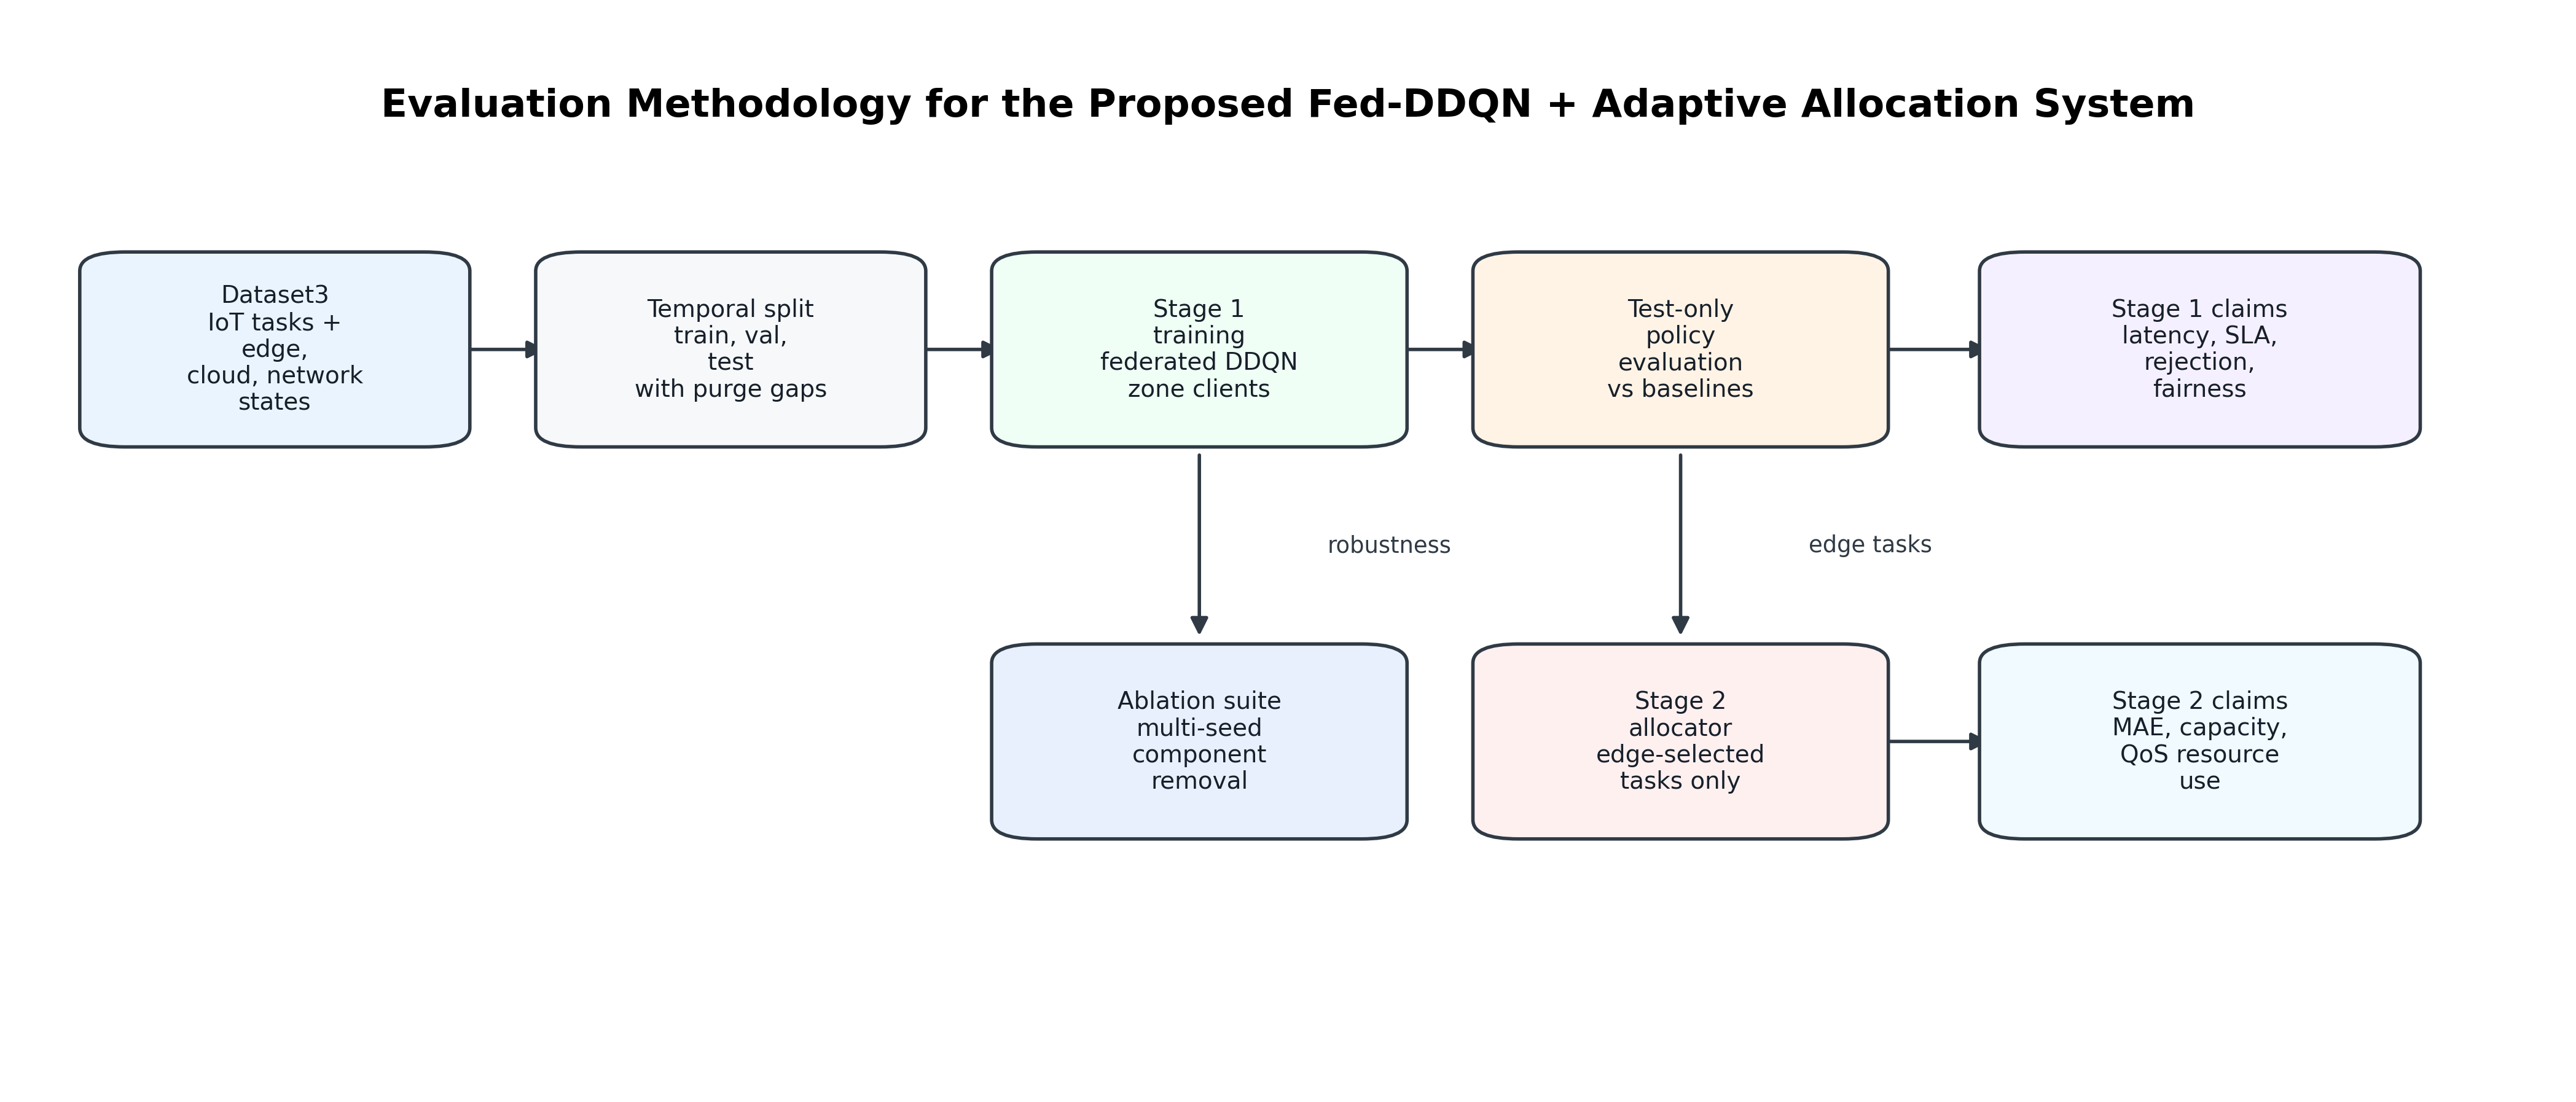
\includegraphics[width=0.90\textwidth]{figures/diagrams/169_fig_a22_experimental_methodology_flowchart.png}
\caption{Experimental flow from label generation through purged temporal splitting, federated training, validation checkpointing, test-only comparison, and Stage-2 allocation.}
\label{fig:methodology_flow}
\end{figure*}

\subsection{Learning Dynamics and Complexity}

The communication cost of one federated round is proportional to the number of participating zones and the number of model parameters:
\begin{equation}
\mathcal{B}_{r} \approx 2Z|\theta|b,
\label{eq:comm_cost}
\end{equation}
where $b$ is the number of bytes per parameter and the factor of two accounts for download and upload. This expression measures model-transfer volume per round, not a universal byte-saving claim. Federated training avoids pooling raw zone records, but the total bytes can exceed one-time raw-feature transfer depending on $Z$, $|\theta|$, the number of rounds, parameter precision, compression, and secure-aggregation overhead.

\begin{figure}[!t]
\centering
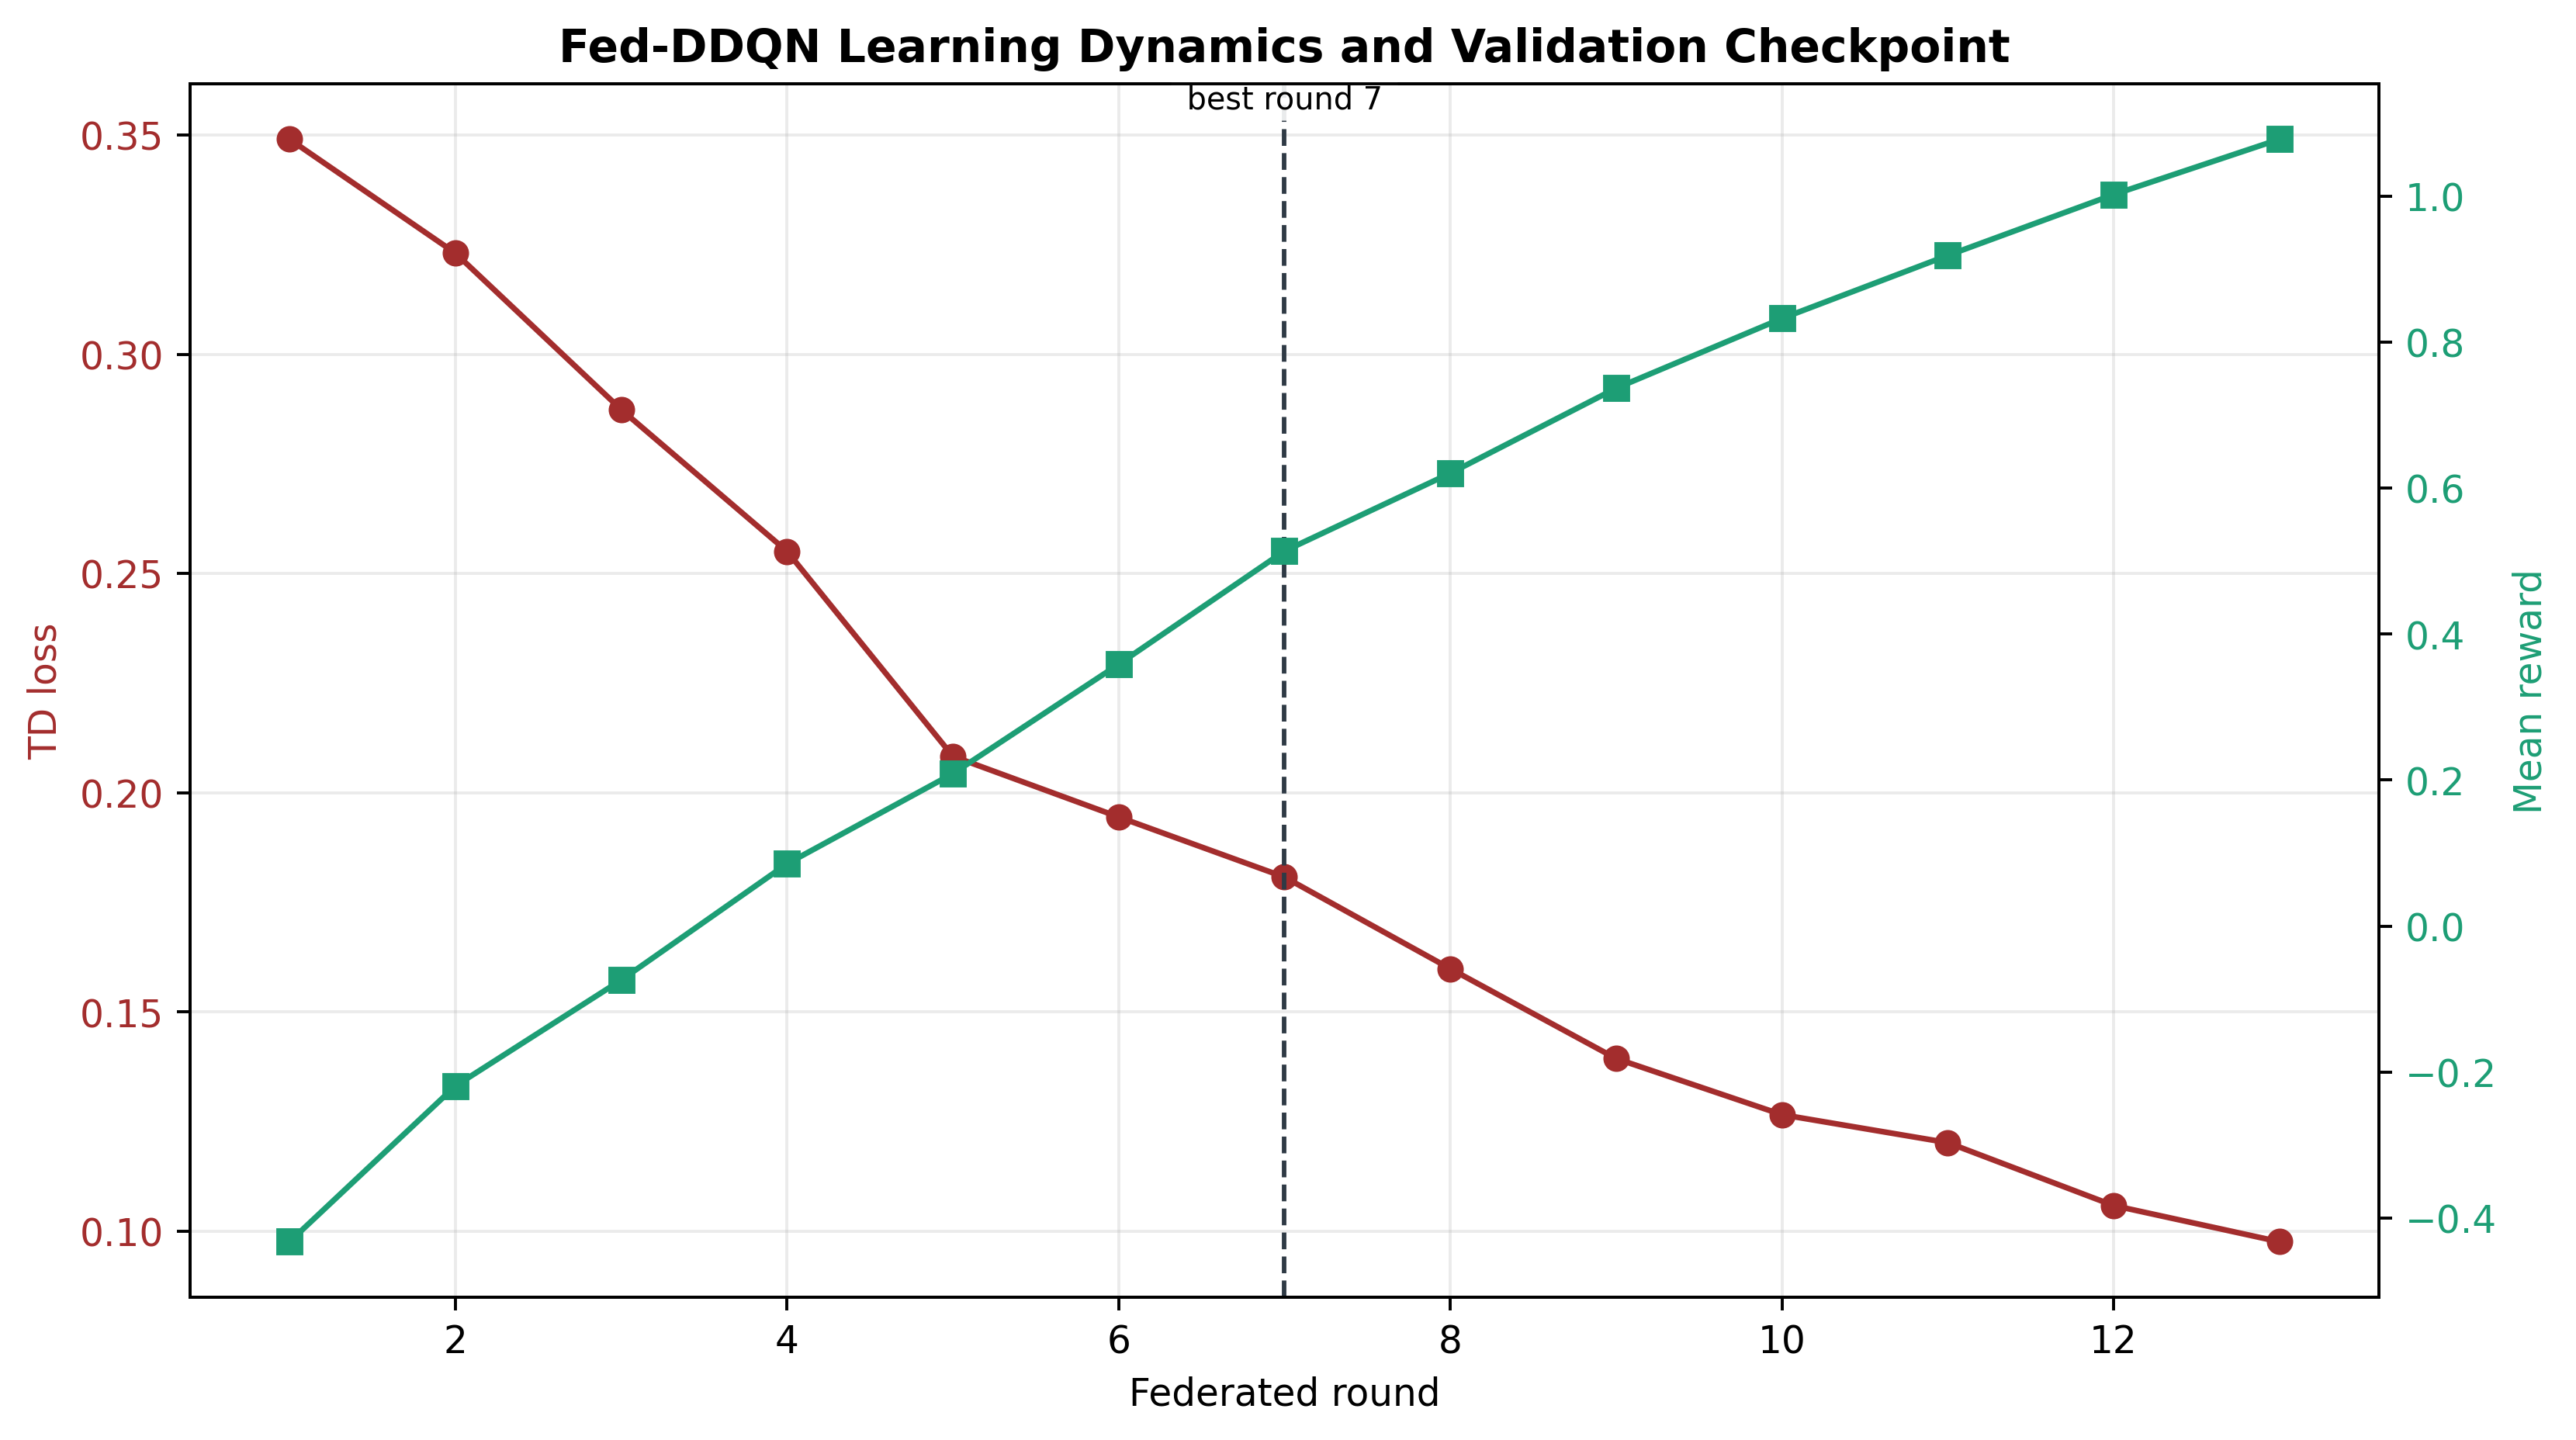
\includegraphics[width=\columnwidth]{figures/diagnostics/162_fig_a13_fed_ddqn_learning_dynamics.png}
\caption{Learning dynamics for the proposed federated policy. The selected checkpoint is based on validation score rather than final training loss alone.}
\label{fig:learning_dynamics}
\end{figure}

The training design is not only about decentralization. It lets the model learn from zone-specific behavior without assuming that every region has the same task mix or channel profile. This motivates the federated DDQN formulation instead of a centralized DDQN with a larger feature vector.

\subsection{Design Rationale}

The final design follows a simple rule: keep the reinforcement-learning action space focused on the edge/cloud choice, and push resource assignment into the second stage. Adding more mechanisms to Stage 1 does not automatically improve the complete objective. Action-aware pressure and prioritized replay can make training more aggressive, but they also change the latency--SLA--rejection balance. The proposed configuration keeps the Fed-DDQN core and uses a conservative training recipe selected by validation performance.

Three implementation choices matter for reproducibility. First, the environment is evaluation-aligned: the reward is computed against the same latency and rejection logic used in final comparison. Second, the validation score combines latency, SLA miss, and rejection instead of choosing the lowest training loss. Third, the test comparison is batched after policy inference, so plots and scenario tables reuse the same actions. These details make the final numbers easier to reproduce and audit.

The design also avoids a tempting shortcut. One could add a rejection action and let the policy reject difficult tasks directly. That would simplify training, but it would make the reported rejection rate partly a policy preference rather than an outcome of infeasibility. The implementation keeps the harder binary action setting: if a task fails, the failure is counted against the selected edge or cloud decision.
